\documentclass[12pt,pdf,hyperref={unicode}]{beamer}
\usetheme{Pittsburgh}
\usecolortheme{seagull}
\usefonttheme{serif}
\usepackage[T2A]{fontenc}
\usepackage[utf8]{inputenc}
\usepackage[english]{babel}
\usepackage{amssymb,amsfonts,amsmath,mathtext}
\usepackage{cite,enumerate,float,indentfirst}
\usepackage{graphicx} 
\graphicspath{{images/}}
\setbeamertemplate{caption}[numbered]
\newcommand\Fontvi{\fontsize{6}{7.2}\selectfont}

\usepackage{geometry} %способ ручной установки полей
\geometry{top=0cm} %поле сверху
\geometry{bottom=0.5cm} %поле снизу
\geometry{left=1.0cm} %поле справа
\geometry{right=0.3cm} %поле слева

\usepackage{hyperref}
\hypersetup{
    colorlinks=false,
    linkcolor=blue,
    filecolor=magenta,      
    urlcolor=cyan,
}

\usepackage{comment}
 \usepackage{pgf} 

\hypersetup{pdfpagemode=FullScreen}
\setbeamertemplate{navigation symbols}{}

\setbeamertemplate{itemize items}[default]
\setbeamertemplate{enumerate items}[default]

\titlegraphic{
\includegraphics[width=4.0cm,height=.14\textheight]{bi-logo}}
\title{Assembly of mammalian genomes using GemCode data }

\author[Кектеева Ангира]{Кектеева Ангира\\{\small \vspace{1cm}   Руководители: Иван Толстоганов, \\Антон Банкевич}}

\date{16 декабря 2017}

\begin{document}
\maketitle

\begin{frame}
\frametitle{Сборка генома}
\begin{flushleft}
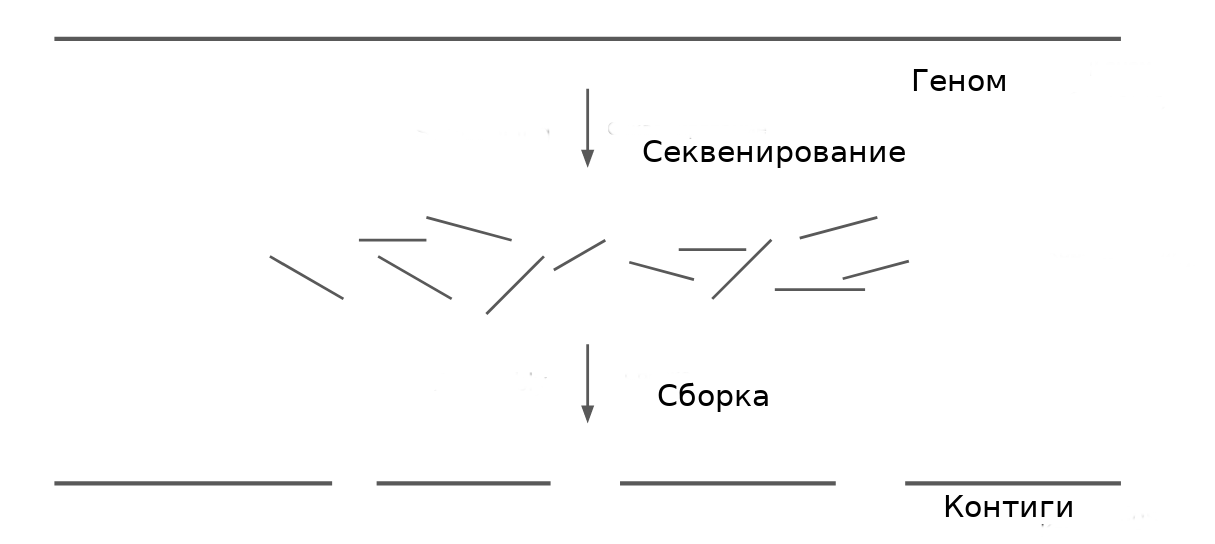
\includegraphics[scale=0.27]{genome_assembly.png}
\end{flushleft}
\end{frame}

\begin{frame}
\frametitle{Облака ридов}
\begin{flushleft}

\includegraphics[scale=0.25]{fragments.png}
\end{flushleft}

Последовательность ДНК "разрезана" на длинные фрагменты.
\end{frame}

\begin{frame}
\frametitle{Облака ридов}
\begin{flushleft}
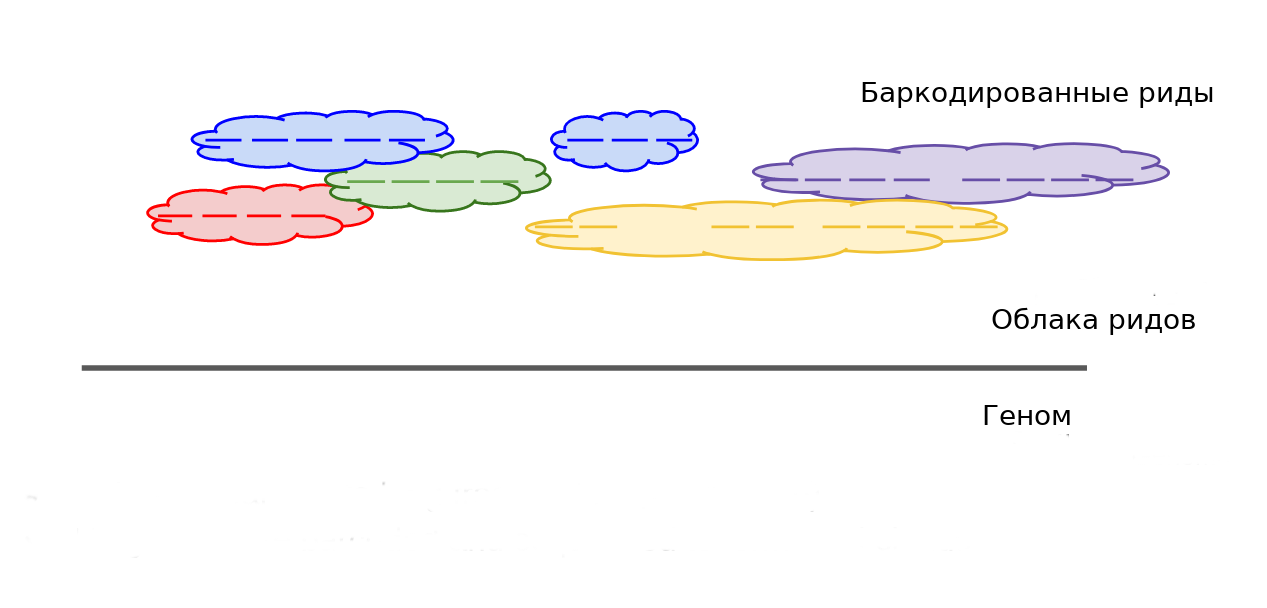
\includegraphics[scale=0.26]{cloud_reads.png}
\end{flushleft}
Фрагменты отмечены баркодами
\end{frame}

\begin{frame}
\frametitle{Задача}
Основной задачей CloudSPAdes является сборка метагеномов, однако используемые в данном инструменте алгоритмы 
разрешения повторов в графе сборки могут быть применены и к сборке млекопитающих. 

\vspace{0.5cm}

Задачи:
\begin{itemize}
\item Изучение существующих алгоритмов сборки с помощью баркодов
\item Анализ недостатков применения текущей стратегии для больших геномов 
\end{itemize}

\end{frame}

\begin{frame}
\frametitle{Проблема повторов}
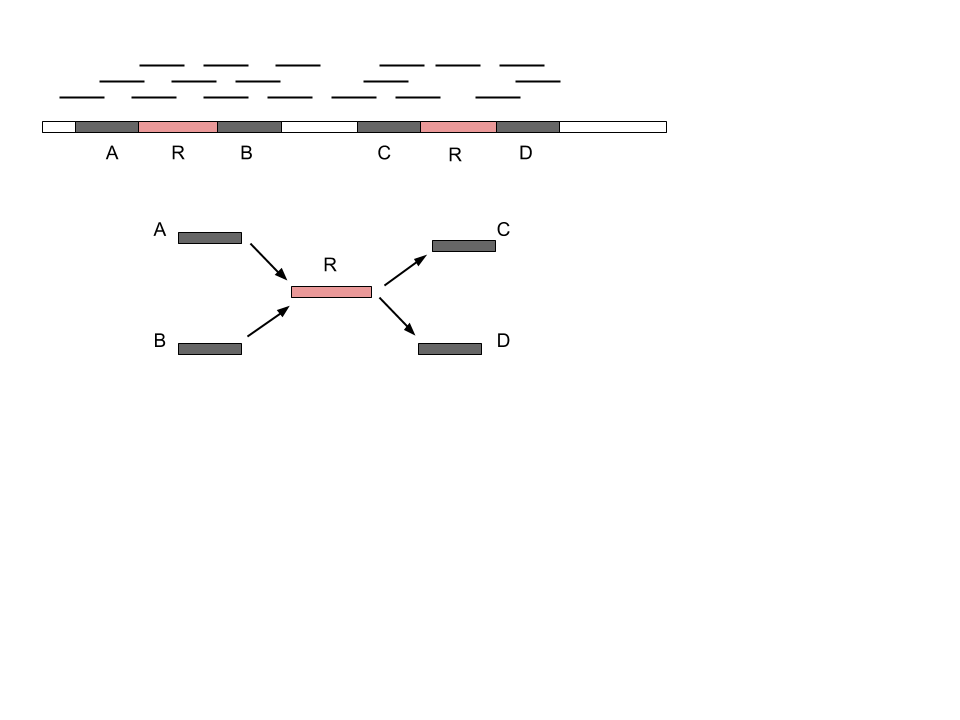
\includegraphics[scale=0.45]{repeats.png}
\end{frame}

\begin{frame}
\frametitle{Геном млекопитающих vs метагеном}

Геном млекопитающих
\center
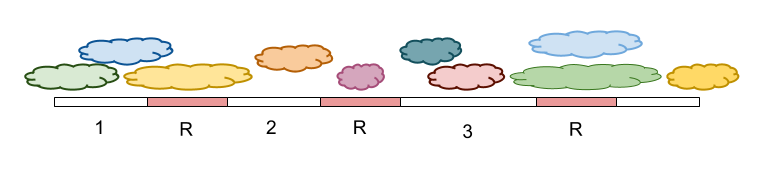
\includegraphics[scale=0.37]{human.png}
\begin{flushleft}
Метагеном
\end{flushleft}

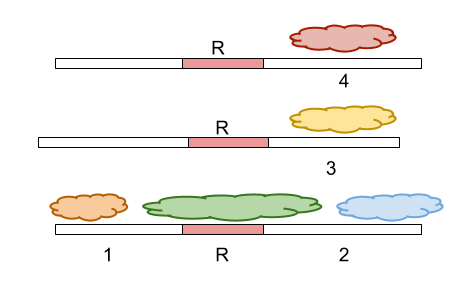
\includegraphics[scale=0.4]{metagenom.png}
\end{frame}

\begin{frame}
\frametitle{Проблема упорядочивания фрагментов генома}
В случае метагеномов сравнительно легко определить порядок следования фрагментов с помощью облаков.
\center
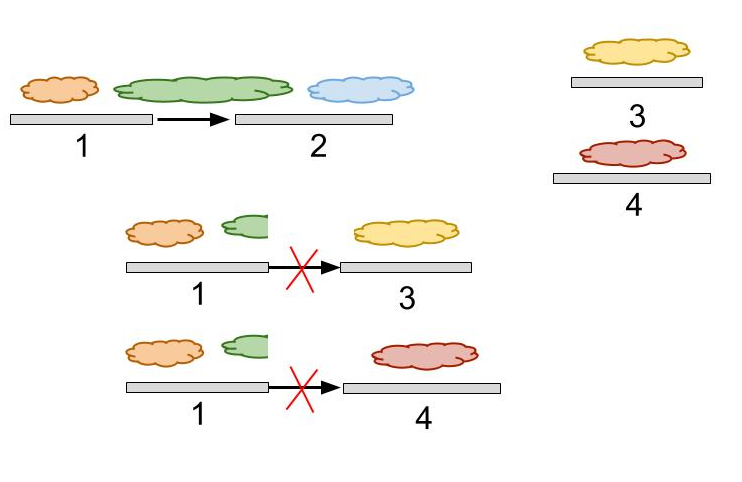
\includegraphics[scale=0.35]{easy.jpg}
\end{frame}

\begin{frame}
\frametitle{Проблема упорядочивания фрагментов генома}
В случае геномов млекопитающих иначе: длинные ребра, связанные повторами в графе, находятся рядом в геноме. 
\center
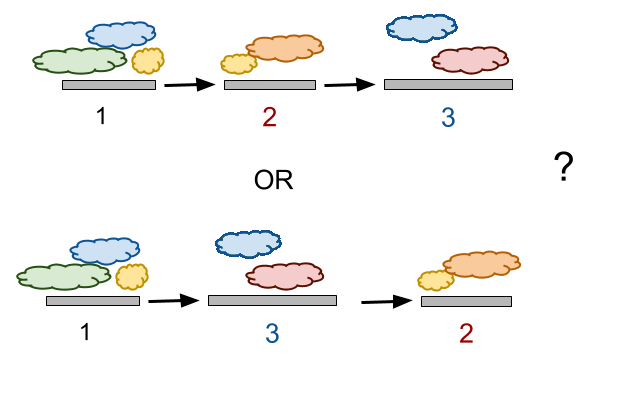
\includegraphics[scale=0.45]{OR.png}
\end{frame}

\begin{frame}
 \frametitle{Близкие рёбра}
 \begin{itemize}
 \item $C(e_1, e_2)$ -- мера схожести наборов баркодов на длинных рёбрах $e_1$, $e_2$
 \item $C(e_1, e_2) = \frac{|E_1 \cap E_2|}{\min(|E_1|, |E_2|)}$
 \item Для некоторого $t$ два ребра $e_1$, $e_2$ считаются близкими, если $C(e_1, e_2) > t$
 \end{itemize}
\end{frame}


\begin{frame}
\frametitle{Среднее количество близких ребер}
\begin{itemize}
 \item $Near(e, t)$ -- доля рёбер, близких к $e$ для данного ребра $e$ и порога $t$ 
 \item Near edge fraction -- среднее $Near(e, t)$ по всем рёбрам
\end{itemize}

\center 
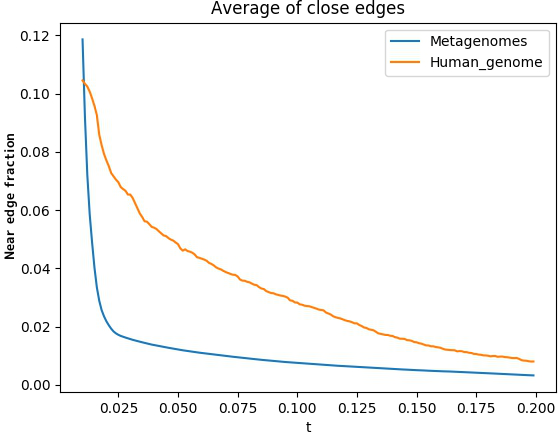
\includegraphics[scale=0.4]{average.png}
\end{frame}

\begin{frame}
\frametitle{Количество ребер с однозначным продолжением}
\begin{itemize}
 \item Unique fraction -- доля рёбер с единственным близким ребром для данного порога $t$
\end{itemize}

\center
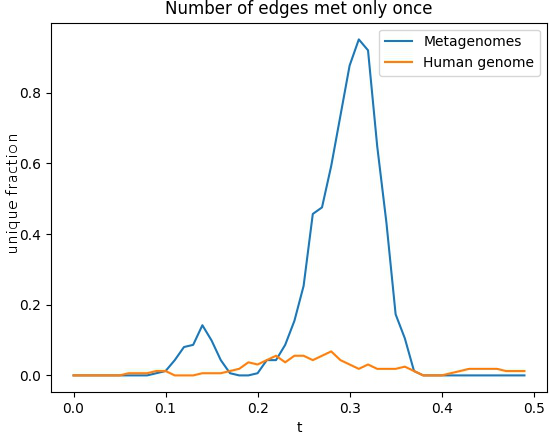
\includegraphics[scale=0.4]{unique.png}

\end{frame}

\begin{frame}
\frametitle{Вывод}
\begin{itemize}
\item Среднее количество близких ребер в человеческом геноме больше, в следствие чего требуется 
разработка дополнительных методов упорядочивания длинных рёбер в геномах млекопитающих.
\end{itemize}
\end{frame}

\begin{frame}
\frametitle{Результаты}
\begin{itemize}
\item Были изучены существующие методы сборки метагеномов с помощью облаков ридов
\item Исследованы недостатки стратегии разрешения повторов применительно к геномам млекопитающих
\end{itemize}
\end{frame}


\begin{frame}
\center
\Large Спасибо за внимание!
\end{frame}

\end{document}
